\section{Bathtub model}
In the previous section we studied the possibility of using a polynomial to capture the relationship between grain size, number of cores, and throughput for a fixed matrix size, with the purpose of finding a range of grain size that leads us to maximum performance. 
Although the polynomial function was helpful in directing us toward our objective, it does not have a physical implication. 

This motivated us to change our view, and instead of looking just at the data and trying to find a function to fit the data, study the behavior of the data, and then find a function that would be likely to fit the data. That function would be a good fit mostly because that's how we expect the throughput to change with grain size, and not just how the data looks like.   

As stated in Section~\ref{task}, Grubel et.al.\cite{grubel2015performance} has studied the task granularity for a specific problem(1D stencil). Looking at the graph representing the execution time based on the grain size, which resembles a bathtub, we are interested in formulating this graph based on our understanding of the effect of task granularity. Figure~\ref{fig21} shows the execution time in terms of grain size for $DMATDMATADD$ benchmark for matrix size $690\times690$ on $4$ cores.

\vspace{\baselineskip}	
\begin{figure}[H]
	\centering
	\subfloat[]{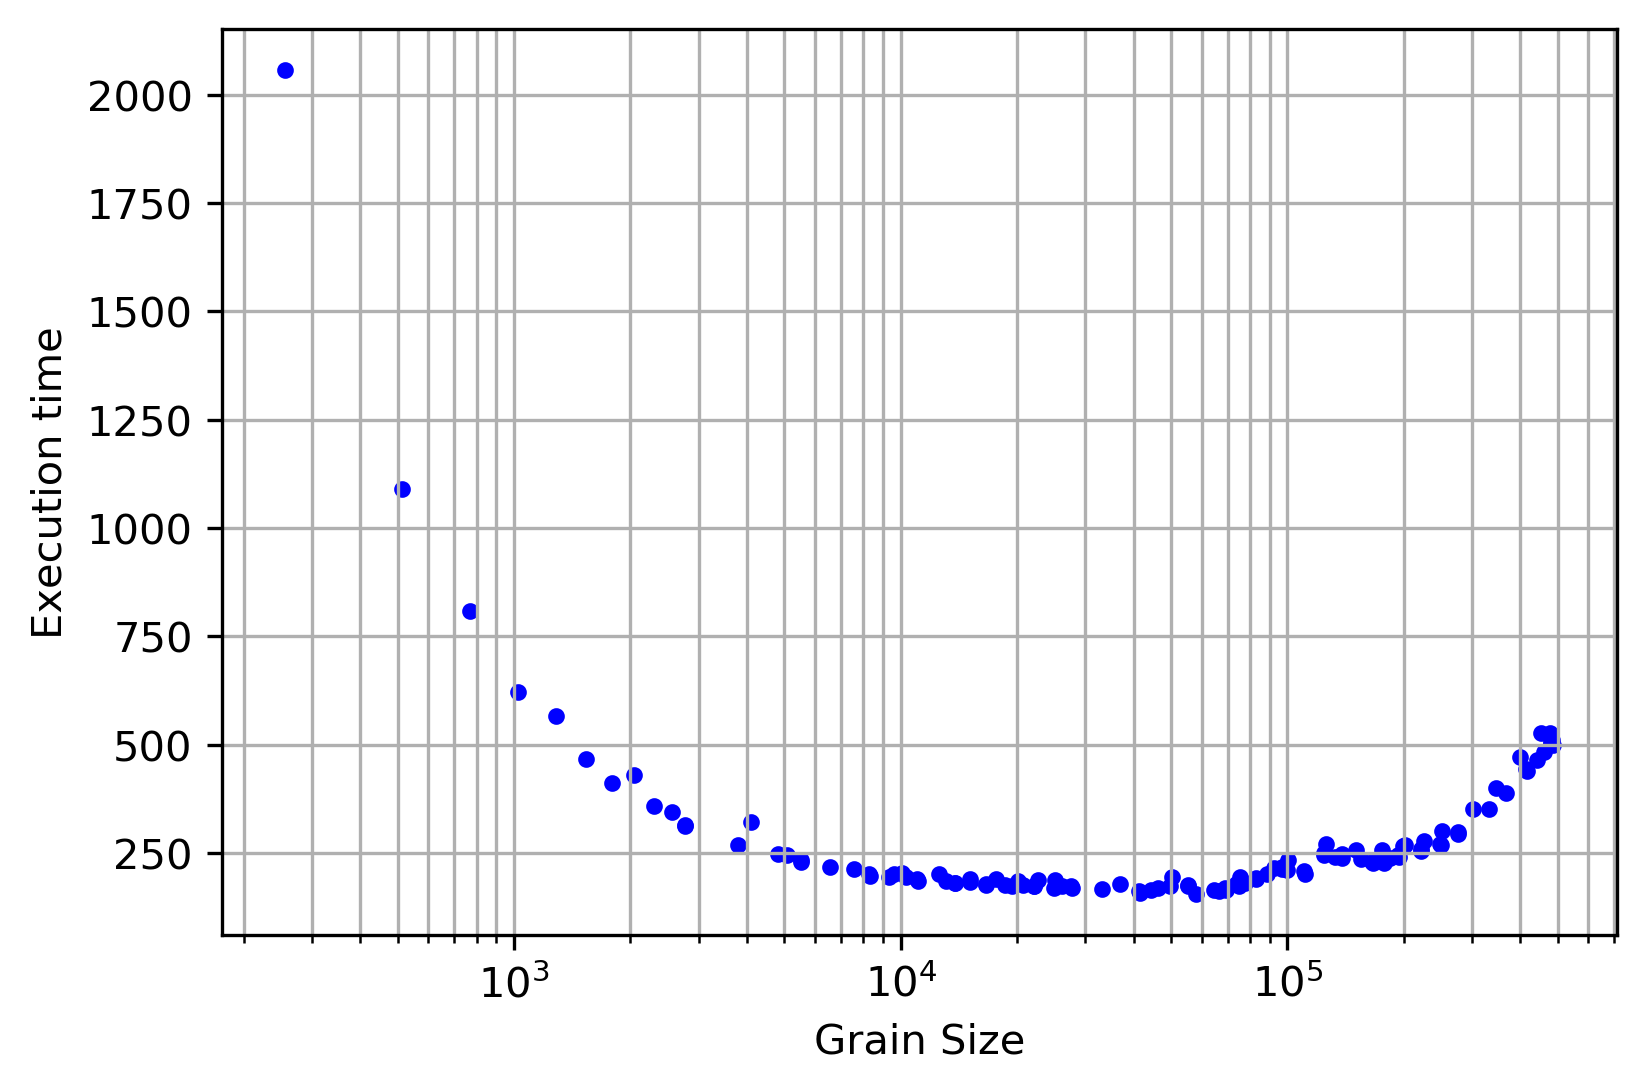
\includegraphics[scale=.5]{images/bathtub/all_690_4.png}\label{fig20:a}}
	\subfloat[]{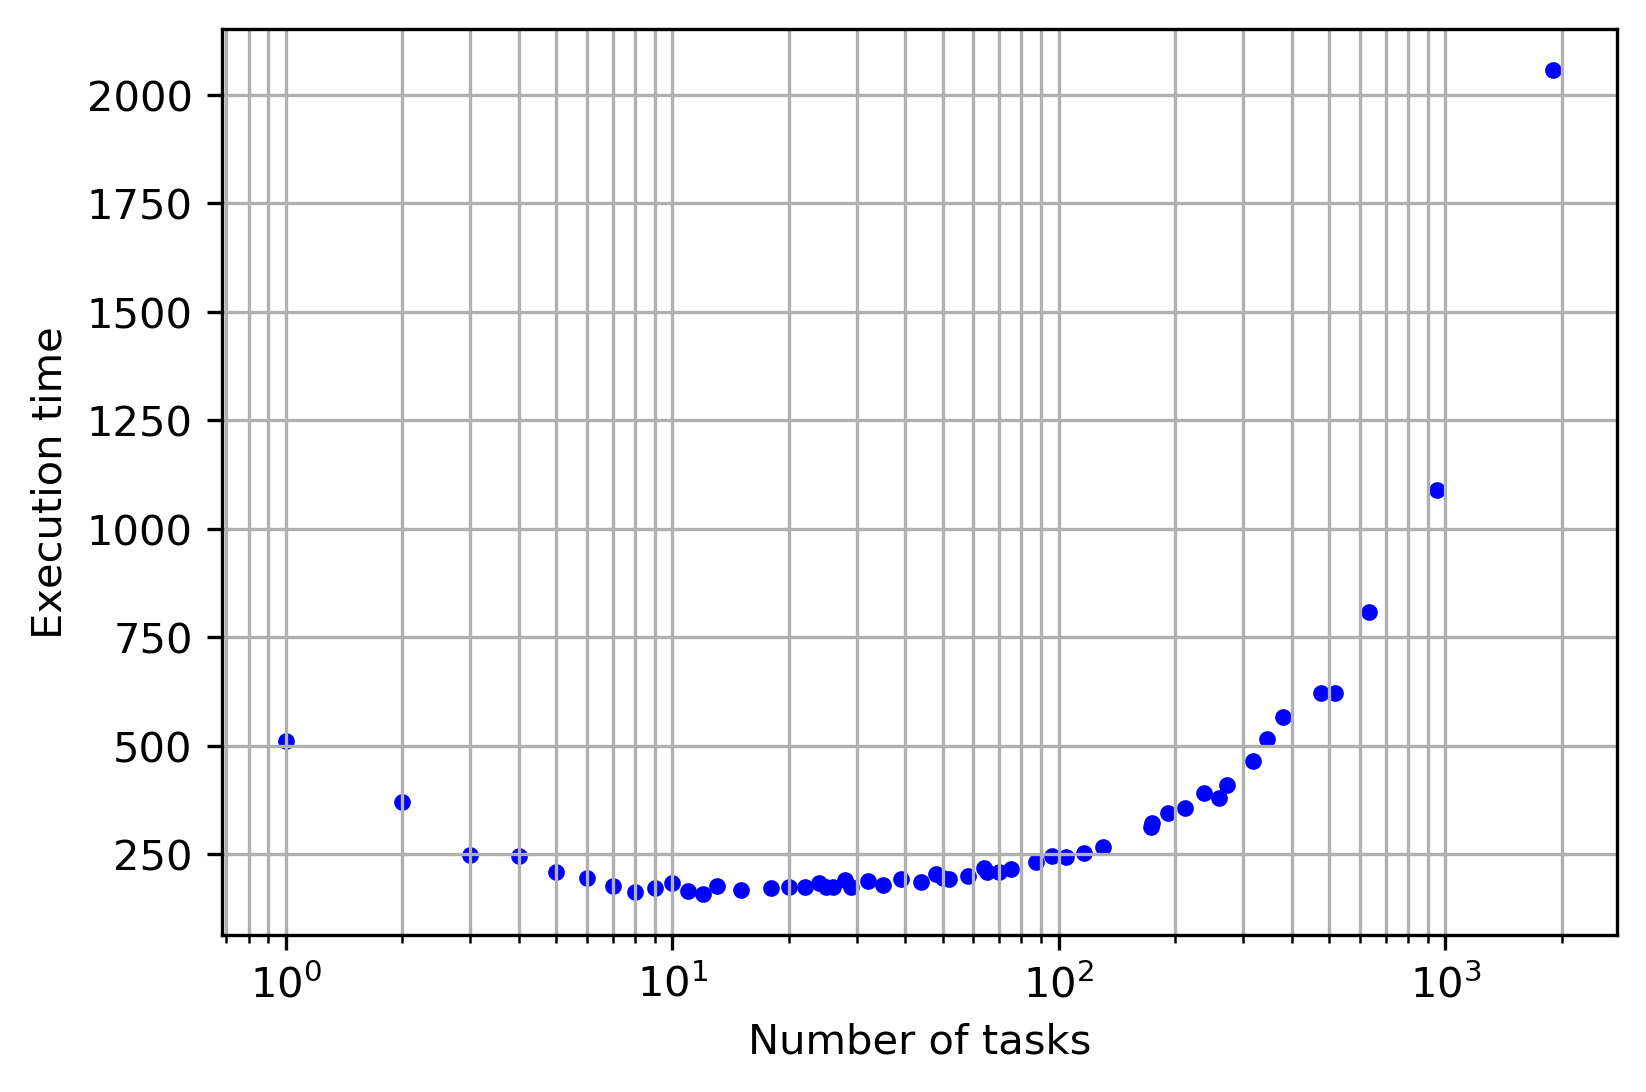
\includegraphics[scale=.5]{images/bathtub/tasks_all_690_4.png}\label{fig20:b}}
	\caption{(a)The execution time vs. grain size graph, and (b) execution time vs. number fo tasks graph for $DMATDMATADD$ benchmark for matrix size $690\times690$ ran on $4$ cores.}	
	\label{fig21}
\end{figure}

\vspace{\baselineskip}	
For the sake of simplicity, we change the x axis from grain size to number of tasks. Each specific grain size would create a specific number of tasks(HPX threads), since the parameters we are interested in are directly associated with he number of tasks, we represent execution time based on number of tasks, as shown in Figure~\ref{fig20:b}.
 

Looking at the left hand side of the graph in Figure~\ref{fig20:b}, we can observe that for the first three points, the number of tasks created is smaller than the number of cores(which is 4 in this example). This means that in any of these cases there is at least one idle core, while the other cores are assigned a rather big chunk of work. The performance degradation we observe in that points is associated with starvation, meaning that we are not utilizing our computation resources to the full extent. In these three points, the number of cores actually doing the work is equal to the number of the tasks, since each core gets to execute at most one task.    

To generalize the problem, assuming we are running our application on $N$ cores, with a grain size equal to $g$, $n_t$ tasks are being created, and $M$ cores are actually doing the work. If $n_t<N$, $M$ would be equal to $n_t$, otherwise $M=N$.


From overhead point of view though, if we represent the overhead of creating one task on a particular machine as $\alpha$, the overhead of creating $d$ tasks would be $n_t\alpha$, but this overhead is divided between the $M$ cores actually doing the work. 

To summarize, knowing the grain size, we are expecting the execution time in a many-task runtime system to be mainly affected by these factors, the overhead of creating one task($\alpha$), the number of cores that are actually doing the work($M$), the sequential execution time($t_s$), and finally the portion of the program that could actually be parallelized($\gamma$). 

If we try to integrate these information into a formula, we would expect the relation between execution time($t$) and number of tasks($n_t$) as follows:
\begin{equation}\label{new}
t=\frac{\alpha{n_t}+t_s}{M}+\gamma
\end{equation}

which could be decomposed into these two equations:

\begin{equation}
t=\left\{
\begin{aligned}
\alpha+\frac{t_s}{n_t}+\gamma  \:\:\:\:\:\:\:\:      \text{ if } n_t<N\\
\frac{\alpha{n_t}+t_s}{N}+\gamma\:\:\:\:\:\:\:\:     \text{otherwise}
\end{aligned}
\right.
\end{equation}

Now we use this function to find the best three parameters $\alpha$, $t_s$, and $\gamma$ so that the collected data would fit this model. For this purpose we used the \textit{curve\textunderscore{fit}} package from \textit{SciPy} library in \textit{python}.

In order to make Equation~\ref{new} differentiable, we used the softplus function(Equation~\ref{softplus}) to represent $M$ based on $n_t$.
\begin{equation}\label{softplus}
f(x)=Ln(1+e^x)
\end{equation}

Which results in Equation~\ref{soft_new}:
\begin{equation}\label{soft_new}
t=\frac{\alpha{n_t}+t_s}{(N-1)-Ln(1+(e^{N-1}-1)e^{-n_t})}+\gamma
\end{equation}

Here again we limited our problem to one specific matrix size at a time, and divided the whole data for each matrix size and number of cores into two parts, $60\%$ for training and $40\%$ for testing.


\vspace{\baselineskip}	
\begin{figure}[H]
	\centering
	\subfloat[]{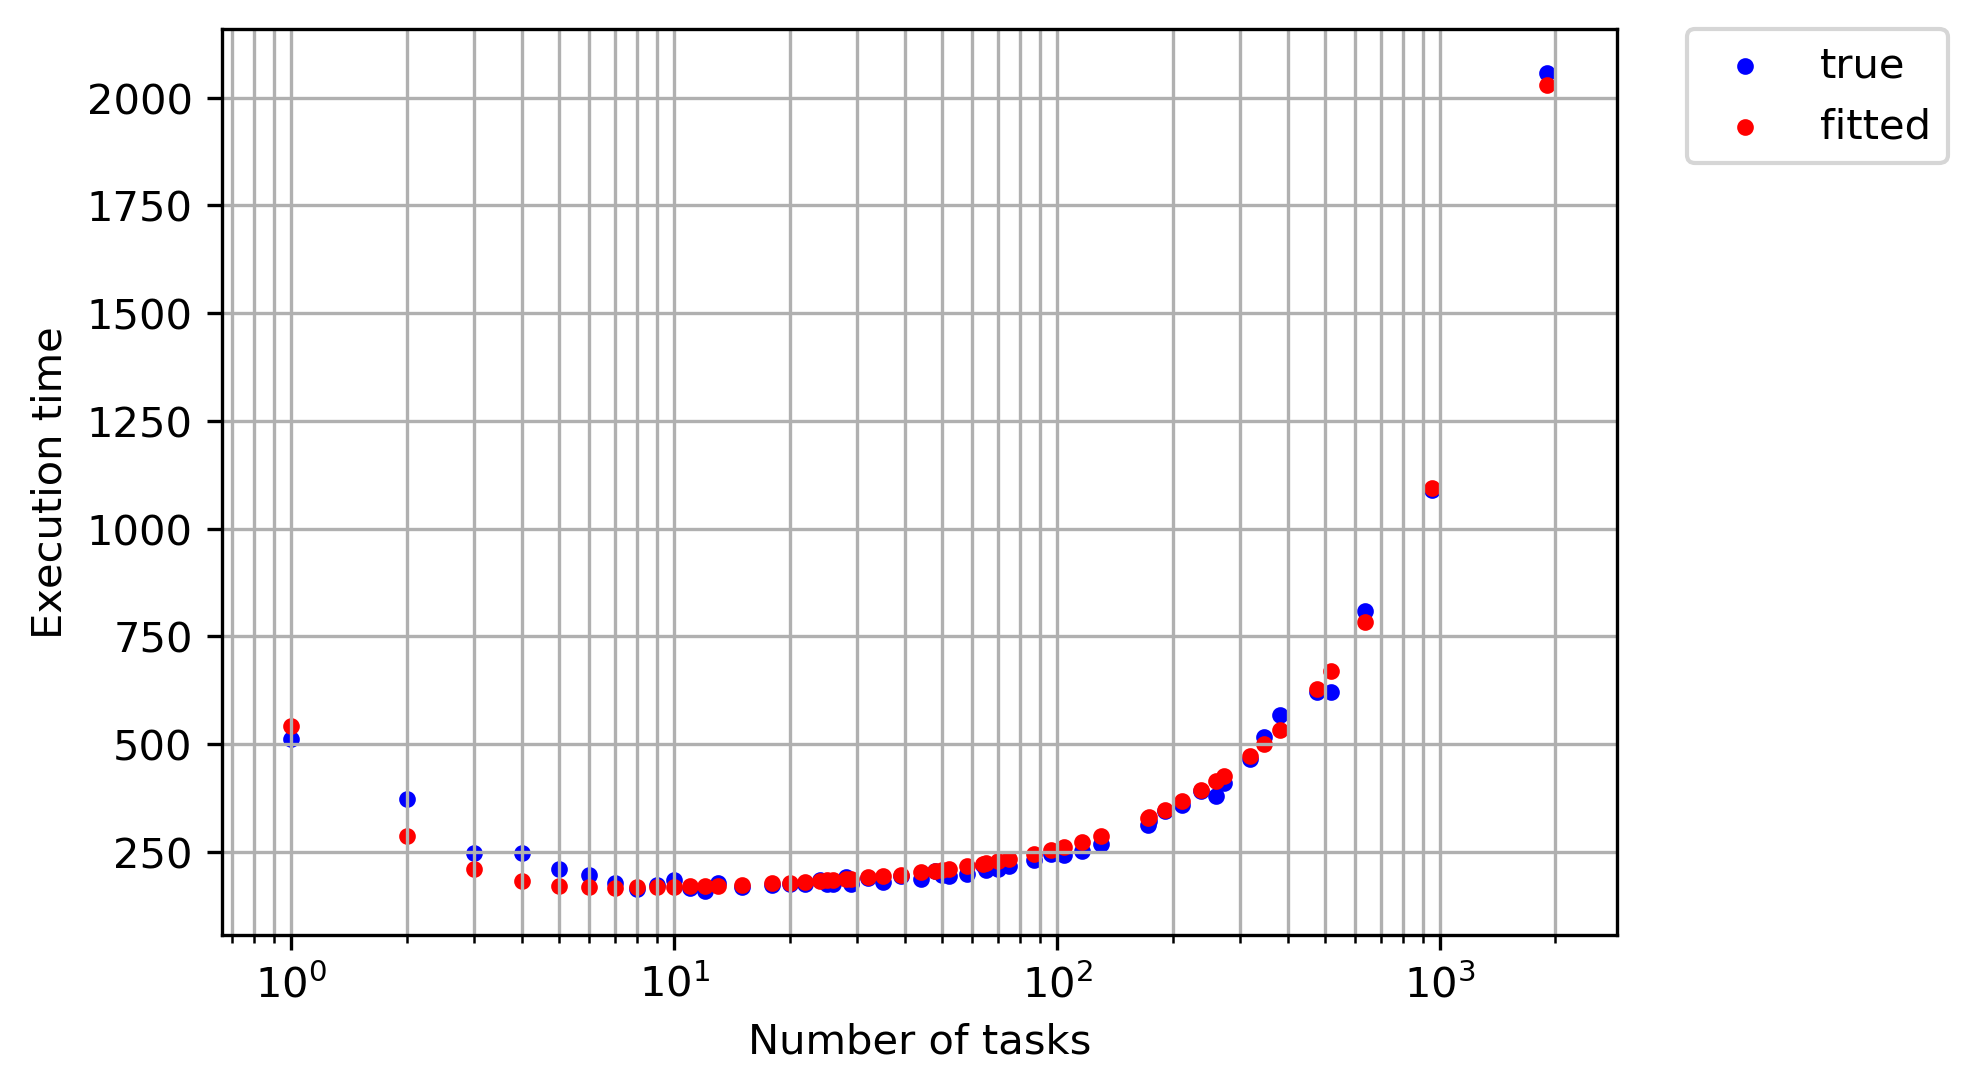
\includegraphics[scale=.45]{images/bathtub/pred/pred_690_4.png}\label{fig22:a}}
	\subfloat[]{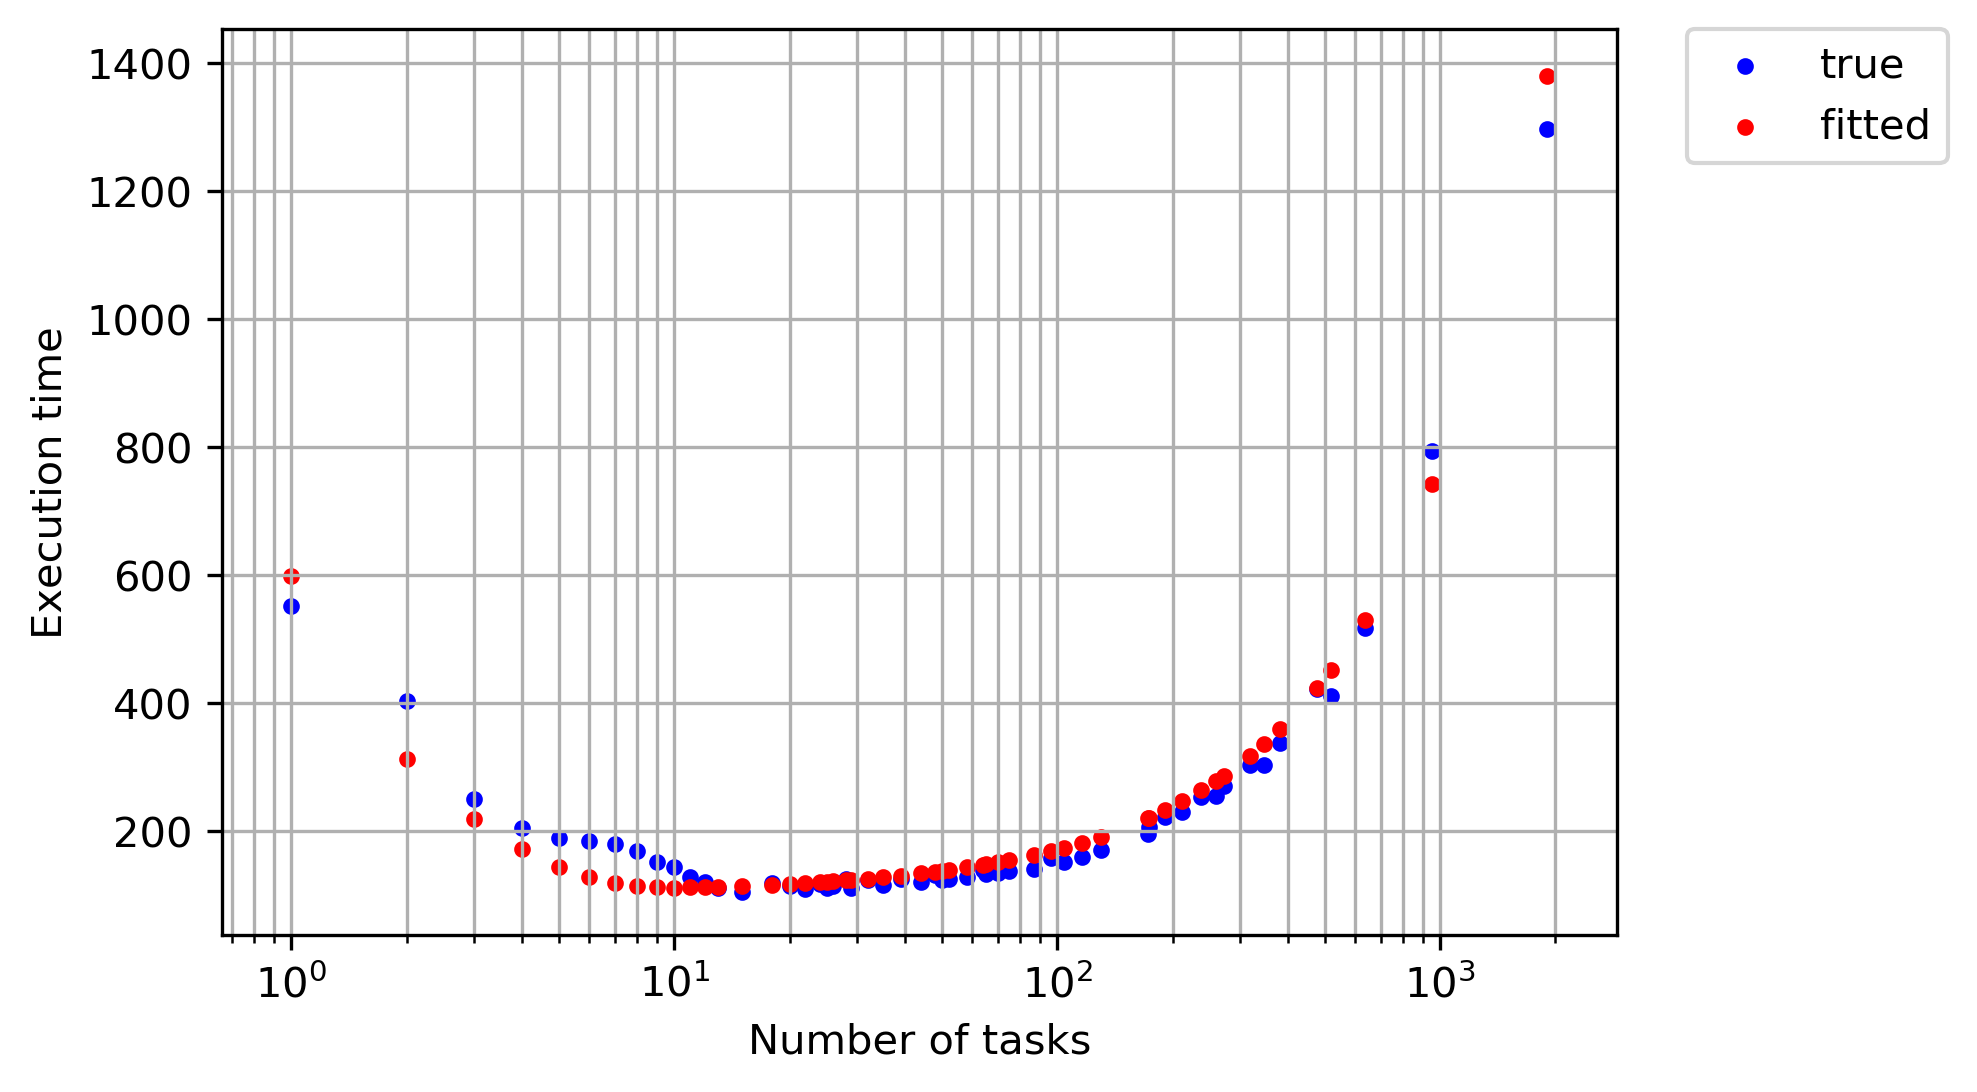
\includegraphics[scale=.45]{images/bathtub/pred/pred_690_8.png}\label{fig22:b}}	
	\caption{The prediction of execution time based on grain size using the bathtub model, for (a)4 cores and (b)8 cores for $DMATDMATADD$ benchmark for matrix size $690\times690$.}	
	\label{fig22}
\end{figure}
\vspace{\baselineskip}	
Figure~\ref{fig23} represents the relative error calculated for both training and test set, which is less than $5\%$.

\vspace{\baselineskip}	
\begin{figure}[H]
	\centering
	{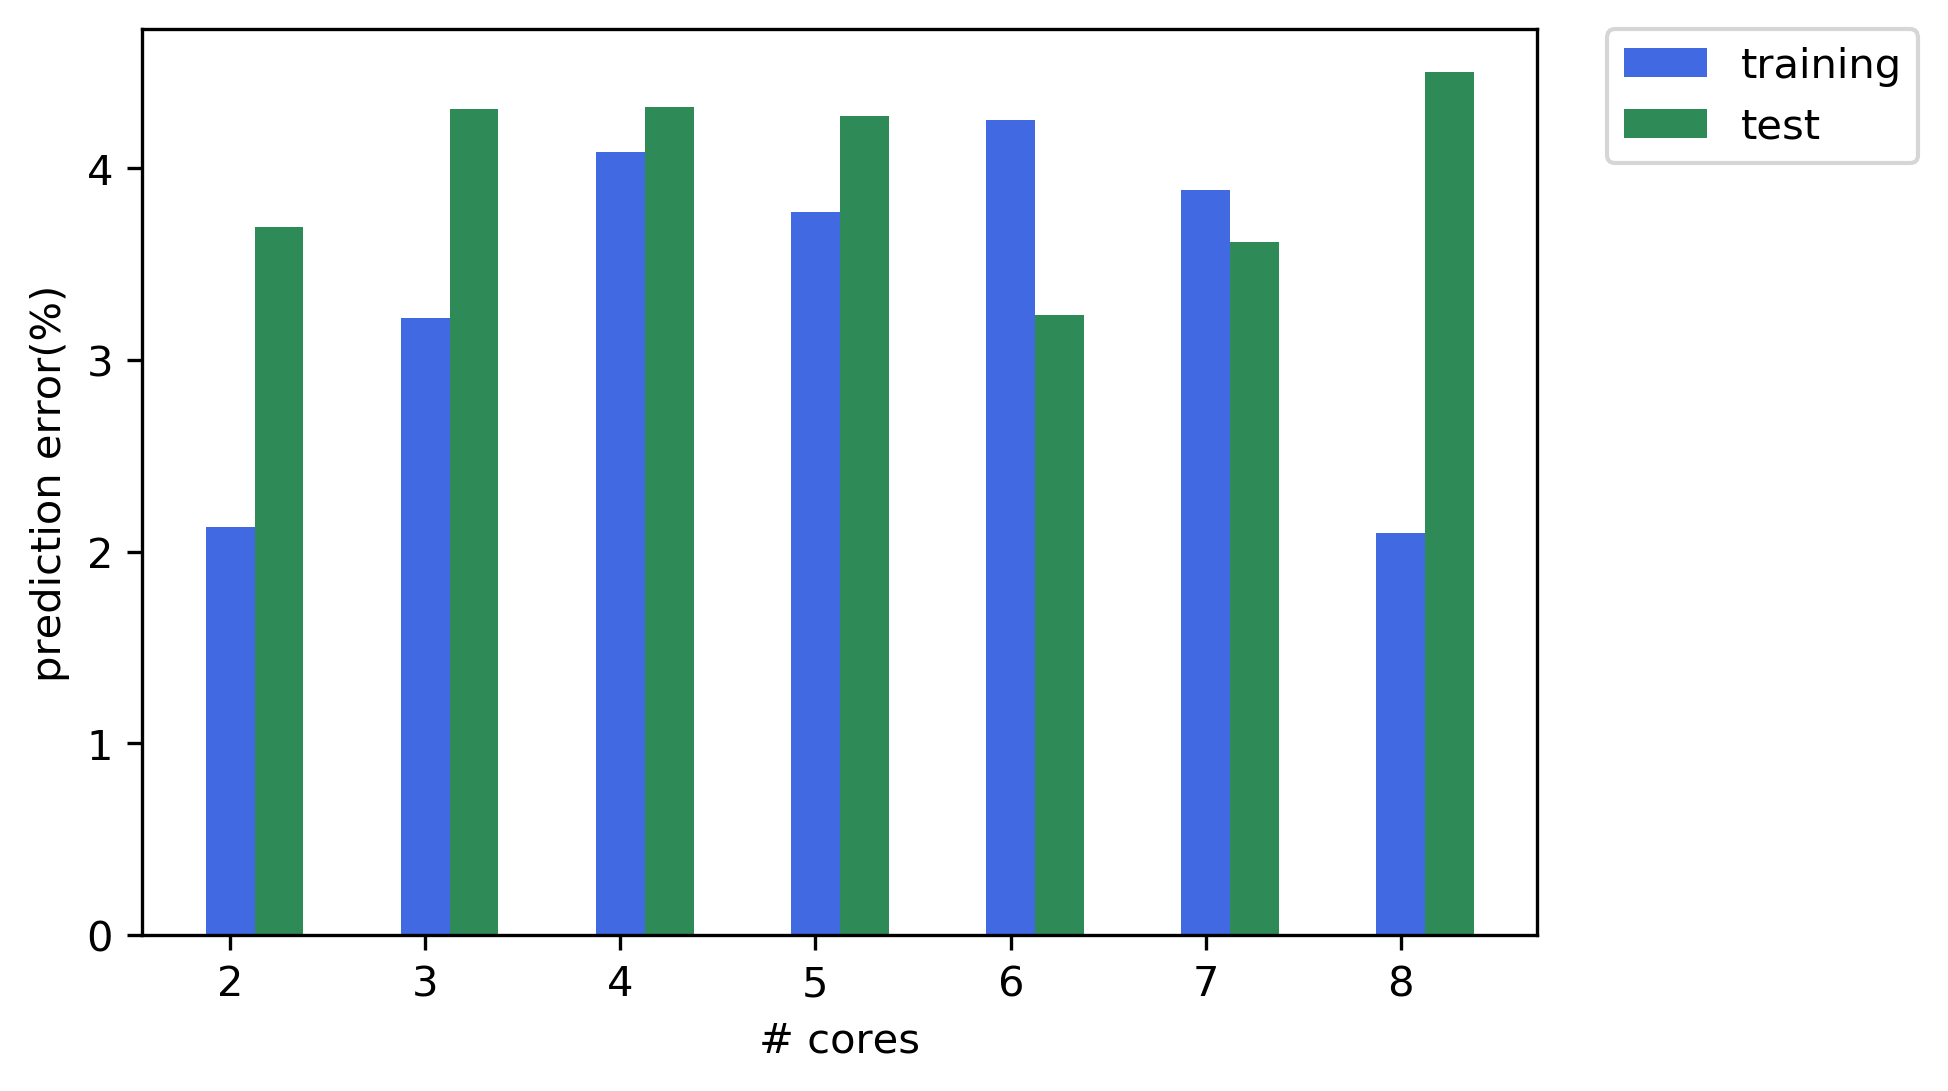
\includegraphics[scale=.45]{images/bathtub/error_690.png}}	
	\caption{The error in fitting execution time with the bathtub formula for $DMATDMATADD$ benchmark for matrix size $690\times690$ with different number of cores.}	
	\label{fig23}
\end{figure}

\vspace{\baselineskip}	
Assuming that this function fits our data in acceptable manner, next step would be to check how these three parameters change with the number of cores.

\begin{equation}\label{usl_fit}
f(x)=\frac{m_0}{x}+\frac{m_1(x-1)}{x}+m_2(x-1)+m_3(x)(x-1)
\end{equation}


\vspace{\baselineskip}	
\begin{figure}[H]
	\centering
	\subfloat[]{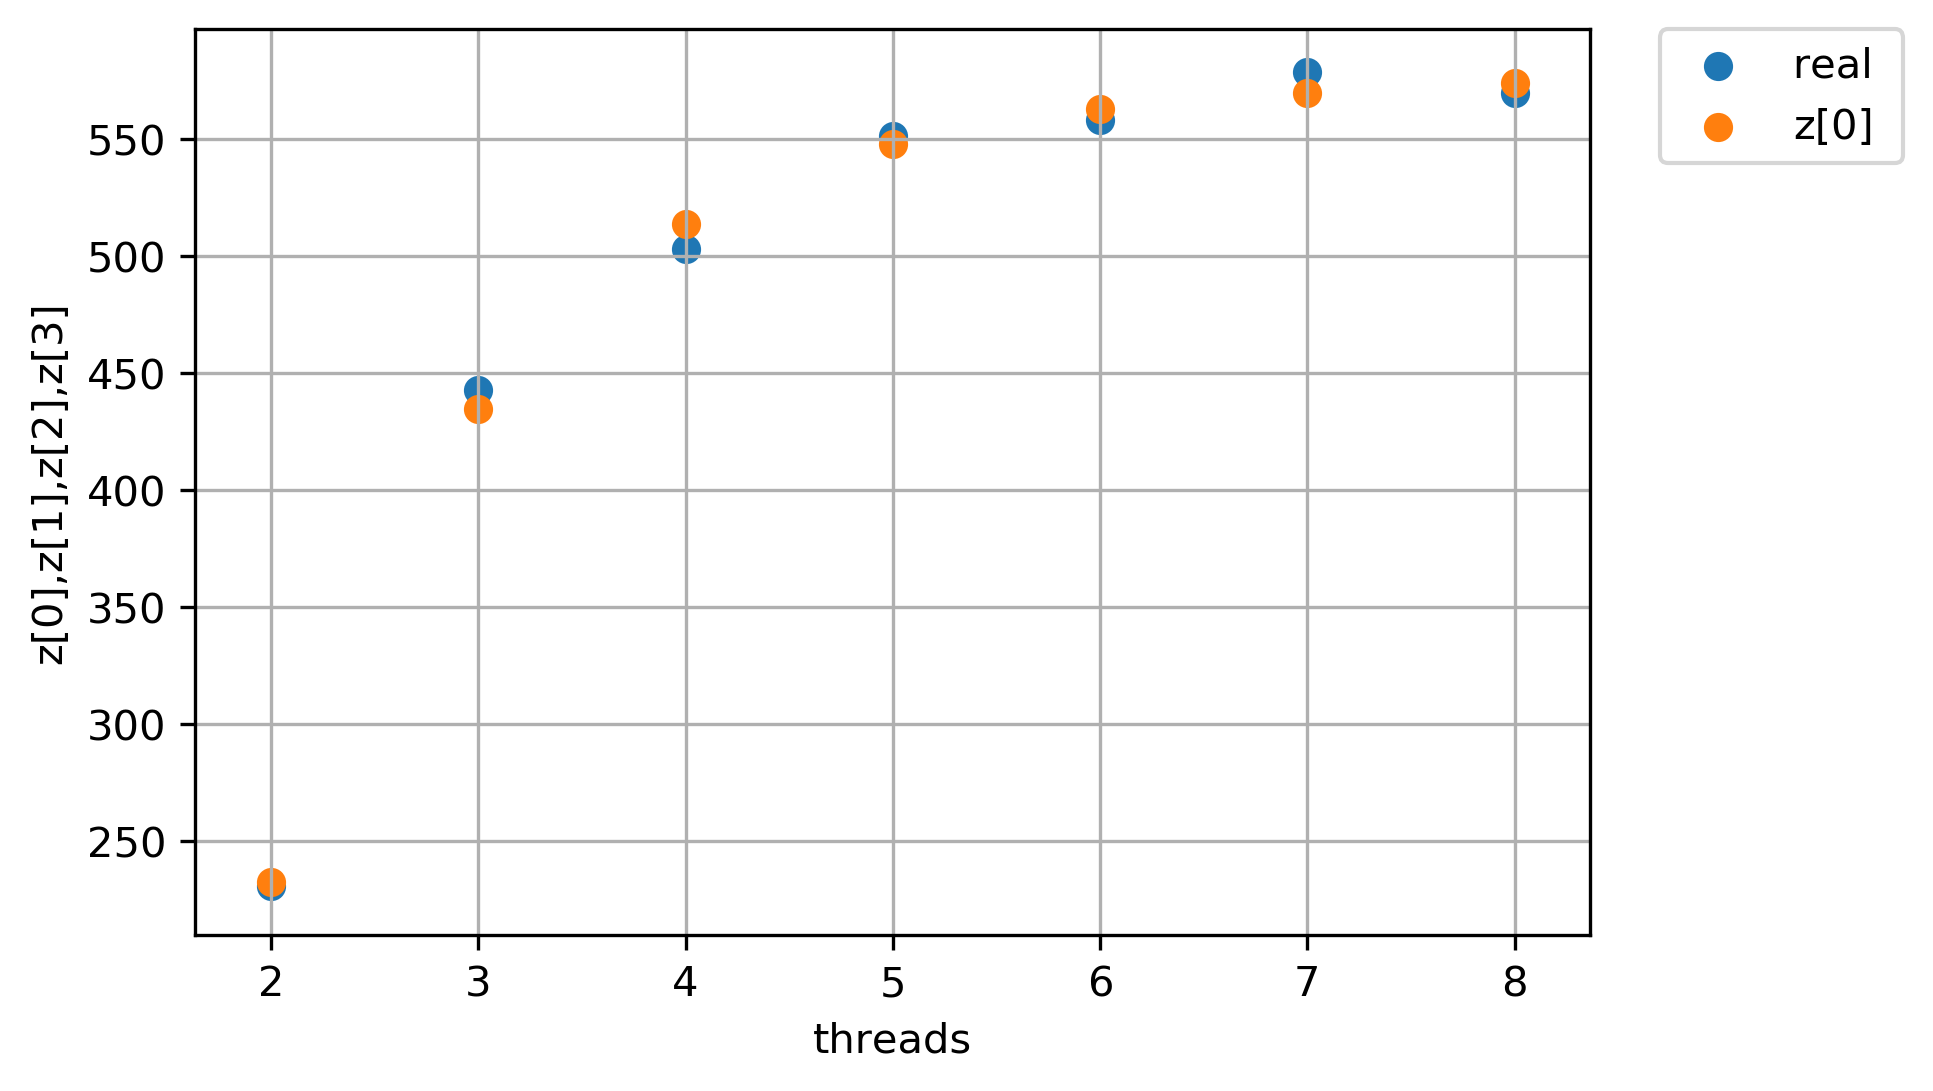
\includegraphics[scale=.3]{images/bathtub/coef_1_690.png}\label{fig24:a}}
	\subfloat[]{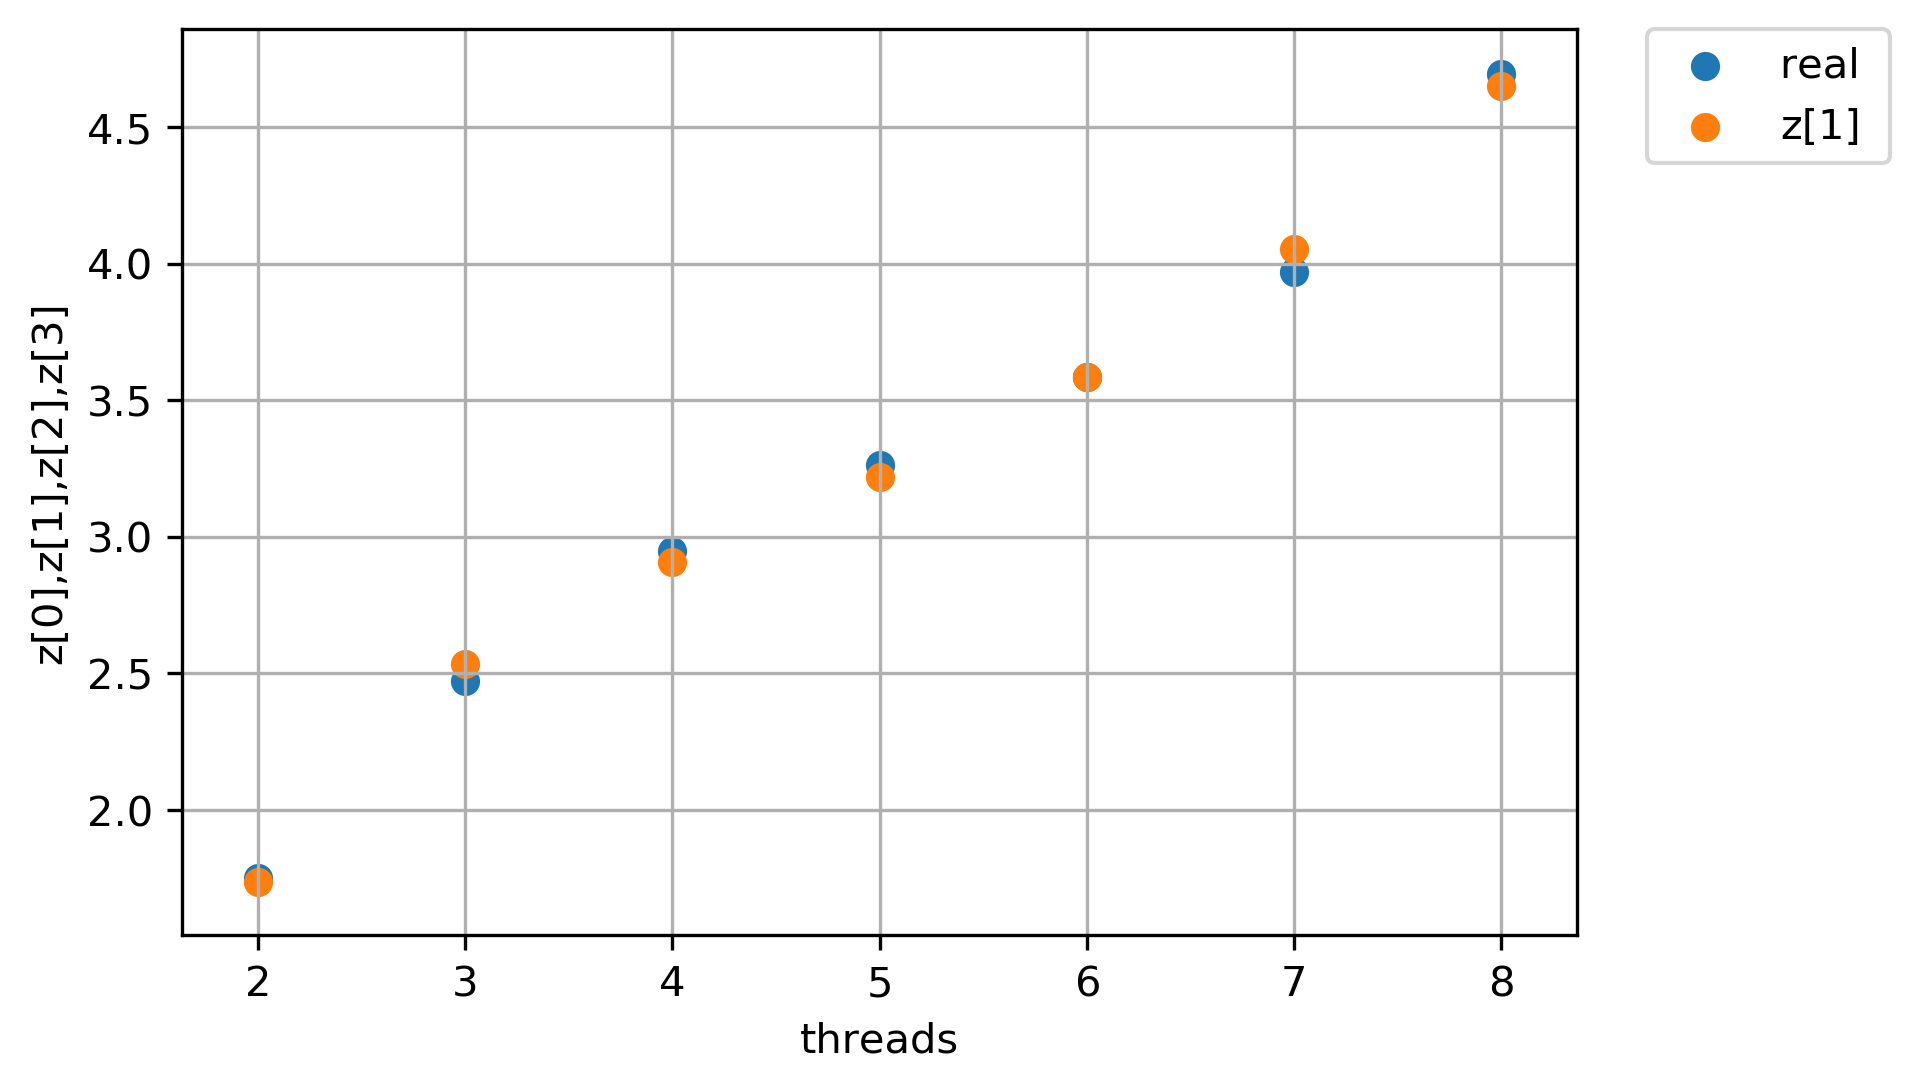
\includegraphics[scale=.3]{images/bathtub/coef_2_690.png}\label{fig24:b}}	
	\subfloat[]{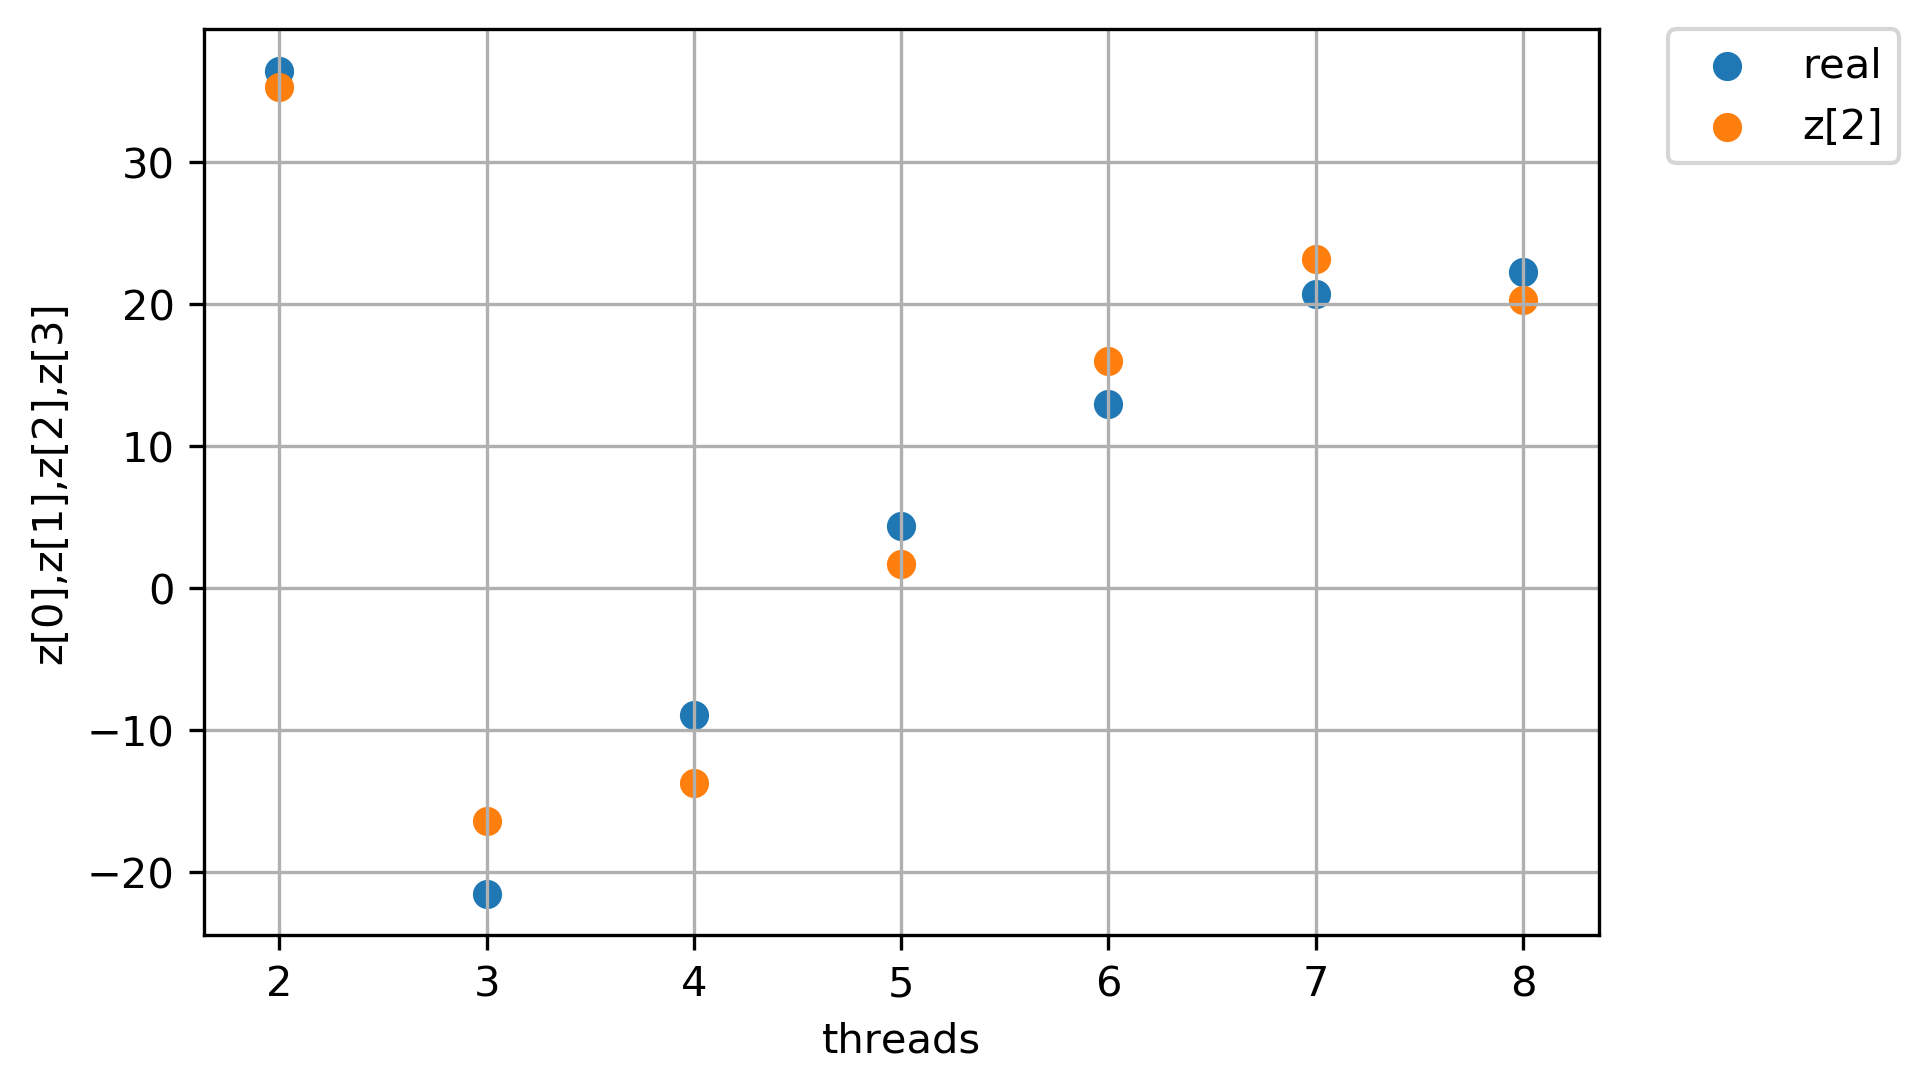
\includegraphics[scale=.3]{images/bathtub/coef_3_690.png}\label{fig24:c}}
	\caption{Fitting the three parameters (a)$\alpha$, (b)$t_s$, and (c)$\gamma$ for $DMATDMATADD$ benchmark for matrix size $690\times690$.}	
	\label{fig24}
\end{figure}


\vspace{\baselineskip}	
We can integrate Equation~\ref{new} and Equation~\ref{usl_fit} to predict the execution time for a given matrix size and number of cores.
For each matrix size having found the parameters $m_0$ to $m_3$, we can find $\alpha$, $t_s$, and $\gamma$ for the particular number of cores requested through Equation~\ref{usl_fit}. Then we can plug in the calculated values for $\alpha$, $t_s$, and $\gamma$ into Equation~\ref{new} to predict the execution time.

Figure~\ref{fig25} shows the prediction error on the test set for $DMATDMATADD$ benchmark for matrix size $690\times690$. The axis shows the different samples in the test set, and the label of each point represents the number of tasks created for that particular data point. As it could be seen, certain number of tasks result in higher prediction error, which needs to be studied.


\vspace{\baselineskip}	
\begin{figure}[H]
	\centering	{\hfill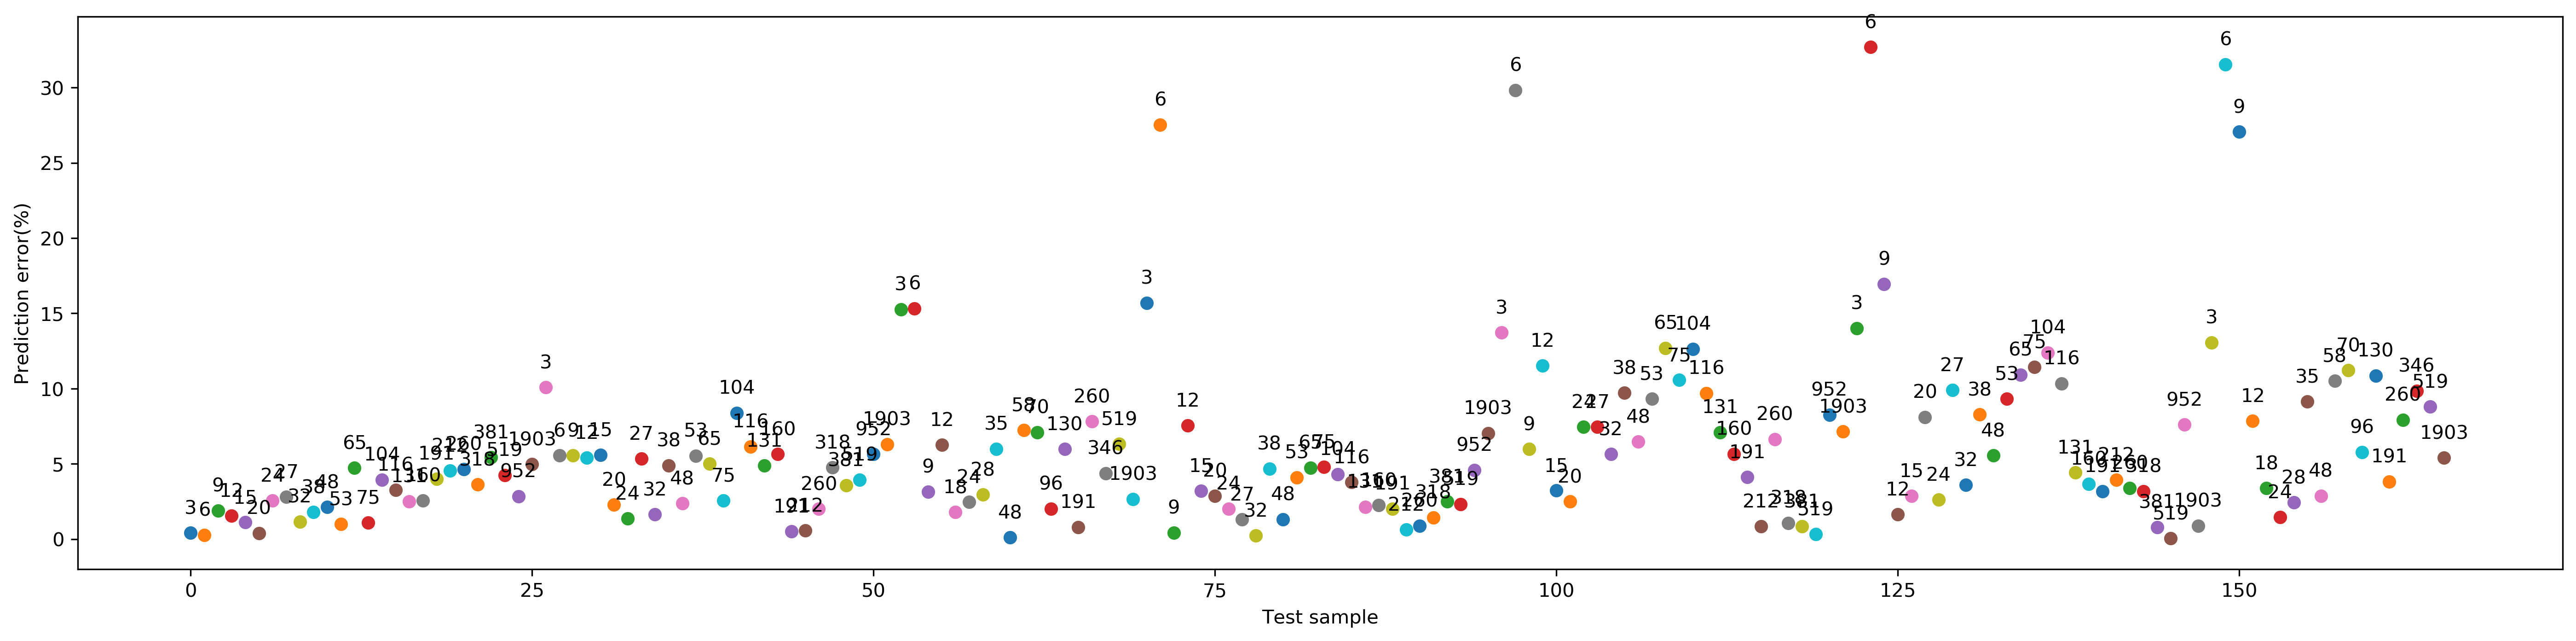
\includegraphics[scale=.35]{images/bathtub/prediction_error_overall690.png}}	
	\caption{The error in fitting execution time with the bathtub formula for $DMATDMATADD$ benchmark for matrix size $690\times690$ with different number of cores.}	
	\label{fig25}
\end{figure}

The problem with the current model is that with this formula we know that the minimum occurs at $n_t=N$, but that's not usually the case. This inspires us to check for a missing factor. 
This model still needs to be studied. The estimate that we have is for execution time, which is in our experiments very small. Changing the graphs from execution time to throughput can help us find the location of the maximum throughput easier compared to minimum of the execution time.


\subsection{Studying the effect of matrix size}

